\section{Governing Equations for a Fluid Model}
\label{sec:fluid_model}

Fluid dynamics may be summarized as the attempt to describe motion of a fluid in a given domain, with given forces and boundary conditions. This section encompasses the derivation of the fluid flow equations, that allows to attempt a solution at this problem. They are the continuity equation (Section \ref{subsec:continuity_eq}) and the Navier-Stokes (Section \ref{subsec:navier_stokes}) equations, which are conservation equations for mass and momentum, respectively. They will be derived from a material standpoint, i.e., following a material point in the fluid. Although it represents a relevant misnomer (indicative of history of continuum mechanics as a subject)\footnote{ As \cite{Truesdell-1954} explains, spatial (Eulerian) and material (Lagrangian) approaches were both considered by Euler before Lagrange. Due to a series of misreports, the material approach is commonly attributed to Lagrange.}, the material approach is typically called Lagrangian approach, and so it will be treated throughout this work. These equations rely on the continuum hypothesis, i.e., they are the result of averaging the discrete, molecular velocities, positions and densities and treating the flow at a coarse scale, from the molecular standpoint. This allows for a description of the medium as a continuum, were these intensive (or bulk) properties vary smoothly at the scale of the flow.

In a domain, flow equations must be solved considering adequate boundary conditions, that are discussed in Section \ref{subsec:boundary_cond}.

An important tool in deriving equations for continuous media is the Reynolds transport theorem. Consider a material system of particles, $\Omega$, with boundary $\partial\Omega$, moving with velocity $\ve{u}(\ve{r})$, where $\ve{r}$ is a position vector. Consider also a spacial domain $\Omega_L$ with boundary $\partial\Omega_L$ \footnote{Herein referring to control volume and control surface, respectively.}, convenient for the purpose of expressing conservation equations. For an intensive quantity $A$, the material derivative of $\int A d\Omega$ is written as
%
	\begin{equation} \label{eq:consv_lagrang}
		\frac{d}{dt}\int_\Omega A(\ve{r},t)d\Omega = \int_{\Omega_L} \frac{\partial A}{\partial t} d\Omega + \oint_{\partial \Omega_L} A \ve{u}\cdot\ve{n} d\Gamma,
	\end{equation}
%
where $t$ is the time, $\ve{n}$ is the outward normal unit vector of the surface element, $d\Gamma$. Applying Gauss' theorem to the previous expression renders
%
	\begin{equation} \label{eq:consv_lagrang_II}
		\frac{d}{dt}\int_\Omega A d\Omega = \int_{\Omega_L} \left( \frac{\partial A}{\partial t} + \ve{\nabla} \cdot(A \ve{u}) \right) d\Omega
	\end{equation}
%
This represents a conservation equation for a given control volume, valid for any quantity $A$, both scalar and vectorial.


%%%%%%%%%%%%%%%%%%%%%%%%%%%%%%%%%%%%%%%%%%%%%%%%%%%%%%%%%%%%%%%%%%%
\subsection{Continuity equation}
\label{subsec:continuity_eq}


In the case of mass conservation, by applying $A=\rho$, Equation \eqref{eq:consv_lagrang_II} is written as
%
	\begin{equation} \label{eq:consv_lagrang_III}
		\int_{\Omega_L} \left( \frac{\partial \rho}{\partial t} + \ve{\nabla}  \cdot(\rho \ve{u}) \right) d\Omega = 0,
	\end{equation}
%
since 
%
	\begin{equation} \label{eq:consv_lagrang_IV}
		\frac{d}{dt}\int_\Omega \rho d\Omega = \frac{dM}{dt} = 0,
	\end{equation}
%
where $M$ is the total mass of $\Omega$, assumed to be conserved in the material system. Expression \eqref{eq:consv_lagrang_III} can be written as 
%
	\begin{equation} \label{eq:consv_lagrang_V}
		\frac{\partial \rho}{\partial t} + \ve{\nabla}  \cdot(\rho \ve{u}) = 0,
	\end{equation}
%
known as the continuity equation of a continuous medium, representing the local conservation of mass. By using the definition of material derivative
%
	\begin{equation} \label{eq:euler_lagrange}
		\frac{dA}{d t}=\frac{\partial A}{\partial t} + \ve{\nabla}  A \cdot \ve{u},
	\end{equation}
%
Equation \eqref{eq:consv_lagrang_V} can be written as
%
	\begin{equation} \label{eq:navier_cont}
		\frac{d \rho}{d t} = - \rho\ve{\nabla} \cdot \ve{u}
	\end{equation}
%

%%%%%%%%%%%%%%%%%%%%%%%%%%%%%%%%%%%%%%%%%%%%%%%%%%%%%%%%%%%%%%%%%%%%%
\subsection{Navier-Stokes equation}
\label{subsec:navier_stokes}

The Navier-Stokes equations represent momentum conservation. Using $A=\rho \ve{u}$, Equation \eqref{eq:consv_lagrang_II} can be transformed in

%
	\begin{equation} \label{eq:ns_I}
		\frac{d}{dt}\int_\Omega \rho \ve{u} d\Omega = \int_{\Omega_L} \left( \frac{\partial \rho \ve{u}}{\partial t} + \ve{\nabla}  \cdot(\rho \ve{u} \ve{u}) \right) d\Omega
	\end{equation}
%
%By grouping the right side of Equation \eqref{eq:ns_I} under $\int_{\Omega_L} \ve{F} d\Omega$, where $\ve{F}$ signifying a force source term for momentum (per unit volume), one obtains
%
%%
%	\begin{equation} \label{eq:ns_II}
%		\int_{\Omega_L} \left( \frac{\partial \rho \ve{u}}{\partial t} + \ve{\nabla}  \cdot(\rho \ve{u} \ve{u}) + \ve{F} \right) d\Omega = 0
%	\end{equation}
%%
%Given that the integral must be zero for any control volume
%
%%
%	\begin{equation} \label{eq:ns_III}
%		\frac{\partial \rho \ve{u}}{\partial t} + \ve{\nabla}  \cdot(\rho \ve{u} \ve{u}) +S_b   = 0
%	\end{equation}
%%
Applying Newton's second law, we can write

%
	\begin{equation} \label{eq:ns_II}
		\frac{d}{dt}\int_\Omega \rho \ve{u} d\Omega = \ve{F}_\Omega,
	\end{equation}
%
where $\ve{F}_\Omega$ represents a force source term for momentum. Expanding the right side of Equation \eqref{eq:ns_I} renders

%
	\begin{equation} \label{eq:ns_IV}
		\ve{F}_\Omega = \int_{\Omega_L} \left(\ve{u}\frac{\partial \rho}{\partial t} + \rho\frac{\partial \ve{u}}{\partial t} + \ve{u} \ve{u} \cdot \ve{\nabla} \rho + \rho \ve{u} \cdot \ve{\nabla}  \ve{u}    + \rho \ve{u} \ve{\nabla}  \cdot \ve{u} \right) d\Omega,
	\end{equation}
%
that can be rearranged into

%
	\begin{equation} \label{eq:ns_V}
		\ve{F}_\Omega = \int_{\Omega_L} \left[ \ve{u}\left( \frac{\partial \rho}{\partial t} + \ve{u} \cdot \ve{\nabla} \rho +\rho \ve{\nabla}  \cdot \ve{u} \right) + \rho\left( \frac{\partial \ve{u}}{\partial t} + \ve{u}  \cdot \ve{\nabla} \ve{u} \right) \right] d\Omega
	\end{equation}
%
Noting that $\ve{u} \cdot \ve{\nabla} \rho +\rho \ve{\nabla}  \cdot \ve{u}\;=\;\ve{\nabla}  \cdot (\rho\ve{u})$ and introducing the continuity equation \eqref{eq:navier_cont}, one obtains the non-conservative, integral form of the momentum conservation equation

%
	\begin{equation} \label{eq:ns_VII}
		\ve{F}_\Omega =  \int_{\Omega_L} \rho\frac{d\ve{u}}{dt}  d\Omega
	\end{equation}
%
For an isolated medium with no external acting forces, total conservation of momentum is then given by $\ve{F}_\Omega=0$. On a general case $\ve{F}_\Omega \neq 0$, meaning that external forces are applied on a control volume $\Omega_L$. These can be written as

%
	\begin{equation} \label{eq:cauchy_I}
		\ve{F}_\Omega = \int_{\Omega_L} \ve{F}_g dm + \oint_{\partial \Omega_L} \ve{T} d\Gamma,
	\end{equation}
%
where $\ve{F}_g$ is the gravitational force (or the resultant of any other body forces) per unit mass and $\ve{T}$ is the contact force, per unit area, on the boundary of $\Omega_L$. Writing the last term as a volume integral by using Gauss' theorem renders

%
	\begin{equation} \label{eq:cauchy_II}
		\oint_{\partial {\Omega_L}} \ve{T} d\Gamma = \int_{\Omega_L} \ve{\nabla}  \cdot \ve{\sigma} d\Omega,
	\end{equation}
%
where $ \ve{\sigma}\cdot\ve{n}=\ve{T} $. Tensor $\ve{\sigma}$ is known as the Cauchy stress tensor and is so that $\sigma_{ij}n_{j}$ is a component of the force being exerted on an surface oriented by $\ve{n}$, per unit area. %The stress tensor effectively represents a momentum flux, with $T$ being the momentum transferred per unit time and unit mass at a given point, trough a unit area normal to $\ve{n}$. 
Since the integral is over an arbitrary fluid element $\Omega_L$, and writing Equation \eqref{eq:cauchy_I} in a local form 

%
	\begin{equation} \label{eq:cauchy_III}
		\frac{d\ve{u}}{dt}=\frac{1}{\rho}\ve{\nabla} \cdot\ve{\sigma} + \ve{g},
	\end{equation}
%
where $\ve{g}$ is the gravitational acceleration vector. The stress tensor can be demonstrated to be symmetrical, Galilean invariant \citep{Aris-1962} and can also be written as a sum of an isotropic tensor and a deviatoric part

%
	\begin{equation} \label{eq:cauchy_IV}
		\ve{\sigma}= -p\ve{I}+\ve{\tau} 
%		\equiv \begin{pmatrix}
%		\sigma_{xx} \;\;\;\;\; \tau_{xy} \;\;\;\;\; \tau_{xz} \\
%		\tau_{yx} \;\;\;\;\; \sigma_{yy} \;\;\;\;\; \tau_{yz} \\
%		\tau_{zx} \;\;\;\;\; \tau_{zy} \;\;\;\;\; \sigma_{zz}
%		\end{pmatrix}
%		=
%		-\begin{pmatrix}
%		p \;\;\;\;\; 0 \;\;\;\;\;0\\
%		0\;\;\;\;\;p \;\;\;\;\;0\\
%		0\;\;\;\;\;0\;\;\;\;\;p 
%		\end{pmatrix}
%		+ 
%		\begin{pmatrix}
%		\sigma_{xx}+p\;\;\;\;\;  \tau_{xy} \;\;\;\;\; \tau_{xz} \\
%		\tau_{yx} \;\;\;\;\; \sigma_{yy}+p\;\;\;\;\; \tau_{yz} \\
%		\tau_{zx} \;\;\;\;\;  \tau_{zy} \;\;\;\;\; \sigma_{zz}+p 
%		\end{pmatrix}
	\end{equation}
%
with

%
	\begin{equation} \label{eq:cauchy_V}
		p=-\frac{1}{3}\text{tr}(\ve{\sigma}) 
		%; \;\;\; \ve{\tau}=\ve{\sigma}+p\ve{I}
	\end{equation}
%
$\ve{I}$ is the identity, $\ve{\tau}$ are deviatoric stresses and the isotropic part is represented by pressure or tensile loads. The separation in isotropic and deviatoric stress tensors is useful for most fluids, since $p$ is an important variable and $\ve{\tau}$ takes known values in specific conditions, for specific fluids\footnote{For example, a Newtonian fluid has $\ve{\tau}=0$ in hydrostatic conditions, as will be discussed in section \ref{subsec:newtonian fluids}.}. The momentum conservation equation can now be written as

%
	\begin{equation} \label{eq:ns_VIII}
		\frac{d\ve{u}}{dt}= -\frac{1}{\rho}\ve{\nabla}p + \frac{1}{\rho}\ve{\nabla}  \cdot\ve{\tau} + \ve{g},
	\end{equation}
%
Equation \eqref{eq:ns_VIII} is open, since the form of the shear stress tensor is not known. It is written in a general form for any continuous medium, and different media require different constitutive equations for the deviatoric stress.


%%%%%%%%%%%%%%%%%%%%%%%%%%%%%%%%%%%%%%%%%%%%%%%%%%%%%%%%%%%%%%%%%%%%%
\subsection{Newtonian Fluids}
\label{subsec:newtonian fluids}

Newtonian fluids represent the simplest fluid model that accounts for viscosity, with fluids like clear water and air being very well represented. The formulation stems from Newton's observation that the shear stress seems to be proportional to the strain rate \citep{Batchelor-2000}, i.e.

%
	\begin{equation} \label{eq:newtonian_fluid_I}
		\ve{\tau} \propto \frac{\partial \ve{u}}{\partial y},
	\end{equation}
%

The mechanism by which stress is exerted by one fluid volume against another finds its explanation at the molecular level. An individual molecule in a fluid executes a random motion, result of thermal fluctuations, bouncing against other molecules, which is superposed on the mean drift motion associated with the flow. Normal stress on a given surface arises from average momentum transfer by the fluid molecules executing their random thermal motion, each molecule imparting an impulse as it collides with the surface and rebounds. Normal stress is exerted even in a static, non-deforming fluid. Generally , shear stress arises when there is a mean velocity gradient in the direction transverse to the flow. Molecules which move by random thermal motion transverse to the flow from a higher mean velocity region toward a lower mean velocity region carry more streamwise momentum than those moving in the opposite direction, and the net transfer of the streamwise molecular momentum manifests itself as a shear stress on the macroscopic level at which we view the fluid.

Three assumptions must be made to derive a form of the shear stresses: i) the shear stress tensor is in fact a linear function of the strain rates; ii) $\ve{\tau}=0$ when the rate of shear is zero (as can be observed by measuring a hydrostatic pressure profile in a water column) and iii) the relationship is isotropic \citep{Batchelor-2000}. Figure \ref{fig:shear_xy} depicts the deformation of a fluid volume as it moves between time $t$ and $t+dt$. 

%
\begin{figure}[ht!]
	\centering 
	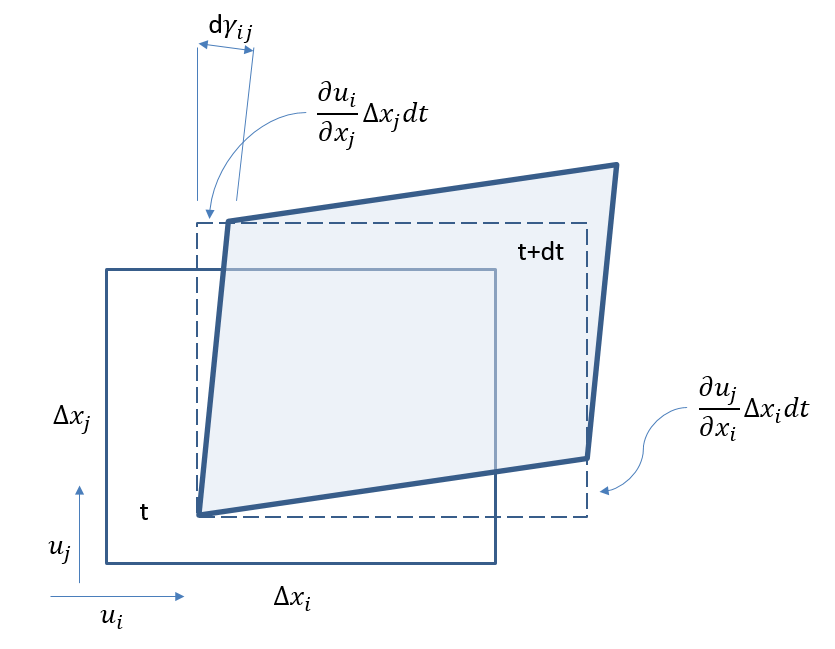
\includegraphics[width=0.65\linewidth]{Figures/2.Chapter/shear_ij}
	\caption{Shear deformation in a fluid volume.}
	\label{fig:shear_xy}
\end{figure}
%

In this interval the shear stress $\tau_{ij}$ produces in the fluid volume an incremental shear strain, $d\gamma_{ij}$, that can be written in a fixed reference frame as 

%
	\begin{equation} \label{eq:shear_strain_I}
		d\gamma_{ij}={\left( \frac{\partial u_i}{\partial x_i} \delta x_i dt \right)}/{\delta x_i}+{\left( \frac{\partial u_j}{\partial x_j} \delta x_j dt \right)}/{\delta x_j}
	\end{equation}
%
In a Lagrangian perspective, the rate of shear strain can be written as

%
	\begin{equation} \label{eq:shear_strain_II}
		\frac{d\gamma_{ij}}{dt}=\frac{\partial u_j}{\partial x_i}+ \frac{\partial u_i}{\partial x_j}
	\end{equation}
%
Imposing assumptions i) and ii), the shear stress is given by

%
	\begin{equation} \label{eq:newtonian_fluid_II}
		\ve{\tau} = \mu \frac{d\gamma_{ij}}{dt}=\mu \left( \frac{\partial u_i}{\partial x_j}+ \frac{\partial u_j}{\partial x_i} \right)=\mu (\ve{\nabla}\ve{u}+ (\ve{\nabla}\ve{u})^T)=2\mu\ve{D} ; \;\;\;\;\;\; (i \neq j)
	\end{equation}
%
where $\ve{D}$ is the strain rate tensor. Assumption iii) imposes that the coefficient of proportionality $\mu$, the shear viscosity coefficient, is the same for any direction and independent from any kinematic quantities. 

Expression \eqref{eq:newtonian_fluid_II} is valid in the case of incompressible flow, where Equation \eqref{eq:navier_cont} is reduced to $\nabla\cdot\ve{u}=0$ and isotropic stresses are not related to shear stresses. If the flow is compressible however, this relationship takes the form of

%%
%	\begin{equation} \label{eq:newtonian_fluid_III}
%		\ve{\tau} = -\left( p_t +\left(\frac{2}{3}\mu - \lambda \right)\ve{\nabla}\cdot\ve{u} \right)\delta_{ij} + \mu \left( \frac{\partial u_i}{\partial x_j}+ \frac{\partial u_j}{\partial x_i} \right)
%	\end{equation}
%%
%
	\begin{equation} \label{eq:newtonian_fluid_III}
		\ve{\tau} = \lambda \text{tr}( \ve{D})\ve{I} + 2\mu\ve{D}
	\end{equation}
%
%where $p_t$ represents the thermodynamic pressure, not the mechanical pressure $p$ and is written as $p_t=p+\lambda\ve{\nabla}\cdot\ve{u}$. The thermodynamic pressure is pressure that would exist if the fluid were in static equilibrium at the local density and temperature. 
where $\lambda$ is another proportionality coefficient, called bulk viscosity\footnote{For the sake of simplicity, the derivation of Equation \eqref{eq:newtonian_fluid_III} was not shown. The details can be consulted on \cite{Batchelor-2000} and \cite{Aris-1962}.}. The effect on the flow of the term which involves the bulk viscosity is usually very small even in compressible flows \citep{Batchelor-2000}. Only when density changes are induced either over extremely small distances (e.g. in the interior of shock waves, where they occur over a molecular scale) or over very short time scales (e.g. in high-intensity ultrasound) will the term involving $\text{tr}( \ve{D}) = \ve{\nabla}\cdot\ve{u}$ be large enough to have a noticeable effect \citep{Zeldovich-1967}.

Disregarding the terms introduced in Equation \eqref{eq:newtonian_fluid_III}, Equation \eqref{eq:ns_VIII} can finally be written as the Navier Stokes equation 

%
	\begin{equation} \label{eq:navier_momentum}
		\frac{d\ve{u}}{dt}= -\frac{1}{\rho}\ve{\nabla}p + \frac{1}{\rho}\mu \ve{\nabla}^2\ve{u} + \ve{g}
	\end{equation}
%




%%%%%%%%%%%%%%%%%%%%%%%%%%%%%%%%%%%%%%%%%%%%%%%%%%%%%%%%%%%%%%%%%%
\subsection{Boundary conditions}
\label{subsec:boundary_cond}


A particular flow problem may be solved by integrating the Navier-Stokes equation, together with the mass conservation equation plus whatever other equations are required to form a complete set, with the boundary conditions appropriate to the particular problem at hand. Equations \eqref{eq:navier_cont} and \eqref{eq:navier_momentum} are applied on a domain $\Omega$, bounded by $\partial\Omega$, composed of solid boundaries $\partial\Omega_B$ and free surfaces $\partial\Omega_F$. A solution yields the velocity components and pressure at the boundaries, from which one obtains the stress tensor via Equations \eqref{eq:cauchy_IV} and \eqref{eq:newtonian_fluid_II}.
In the absence of surface tension, the boundary conditions consistent with the continuum hypothesis are that i) the velocity components and ii) the stress tensor components must be continuous at all points in the domain, including across phase interfaces such as $\partial\Omega_B$ and $\partial\Omega_F$. These conditions can be translated into kinematic and dynamic impositions. The kinematic boundary condition reads

%
	\begin{equation} \label{eq:bc_kinematic}
		\ve{u}|_{\partial\Omega}=\overline{\ve{u}}|_{\partial\Omega},
	\end{equation}
%

where $\overline{\ve{u}}$ corresponds to an imposed velocity. This condition is inherently verified by the Lagrangian framework. The dynamic boundary condition must express ii), i.e., the continuity of stresses across the interface. Such condition is evident to impose at $\partial\Omega_B$

%
	\begin{equation} \label{eq:bc_ns_I}
		\ve{\sigma}|_{\partial\Omega_B}=\ve{\sigma}|_{\partial\Omega}; \;\;\;\;\forall: \partial\Omega_B \in \partial\Omega
	\end{equation}
%
Equation \eqref{eq:bc_ns_I} simply interprets \eqref{eq:cauchy_II} as a boundary condition. The same can be done in the case of the free-surface, typically imposing a given stress tensor, $\overline{\ve{\sigma}}$, at each point:

%
	\begin{equation} \label{eq:bc_ns_II}
		\ve{\sigma}|_{\partial\Omega_F}=(-p\ve{I}+ 2\mu\ve{D})|_{\partial\Omega_F}= \overline{\ve{\sigma}}|_{\partial\Omega_F}
	\end{equation}
%
After normal projections, one can write

%
	\begin{equation} \label{eq:bc_ns_III}
		p=2\mu \ve{n}\cdot\frac{\partial \ve{u}}{\partial\ve{n}}
	\end{equation}
%
where $\ve{n}$ is the unit vector normal to the free surface. This relation implies that the pressure field may be discontinuous at the free surface. 




